\documentclass{article}
\usepackage[top=.5in, bottom=.5in, left=.9in, right=.9in]{geometry}
\usepackage[latin1]{inputenc}
\usepackage{enumerate}
\usepackage{hyperref}
\usepackage{graphics}
\usepackage{graphicx}
\usepackage{caption}
\usepackage{subcaption}
\usepackage{tabularx}
\usepackage{amsmath}
\usepackage{amssymb}
\usepackage{siunitx}
\usepackage{mathtools}
\usepackage{bbm}



\usepackage[authoryear,round]{natbib}

% Use instead of natbib
%\usepackage[backend=bibtex,citestyle=authoryear-comp,natbib=true,sorting=none,hyperref=true,maxnames=2,arxiv=pdf]{biblatex}
%\renewbibmacro{in:}{}
%\addbibresource{/Users/Evan/GitProjects/tex-docs/references.bib}




\newcommand{\obar}[1]{\ensuremath{\overline{ #1 }}}
\newcommand{\iid}{\ensuremath{\stackrel{\textrm{iid}}{\sim}}}
\newcommand{\op}[2]{{\ensuremath{\underset{ #2 }{\operatorname{ #1 }}~}}}
\newcommand{\norm}[1]{{ \ensuremath{ \left\lVert  #1 \right\rVert  }  }}
\newcommand{\cov}{ \ensuremath{ \textrm{cov} } }
\newcommand{\var}{ \ensuremath{ \textrm{var} } }
\newcommand{\tr}{ \ensuremath{ \textrm{trace} } }
\newcommand{\df}{ \ensuremath{ \textrm{df} } }
\newcommand{\R}{ \ensuremath{ \mathbb{R} }}
\newcommand{\indicator}[1]{ \ensuremath{ \mathbbm{1}\left\{ #1 \right\} }   }

\usepackage{xcolor}
\definecolor{darkgreen}{rgb}{0,0.25,0}
\newcommand{\soln}{{\color{red}\textbf{Solution:~}\color{black}}}


\usepackage[formats]{listings}
\lstdefineformat{R}{~={\( \sim \)}}
\lstset{% general command to set parameter(s)
basicstyle=\small\ttfamily, % print whole listing small
keywordstyle=\bfseries\rmfamily,
keepspaces=true,
% underlined bold black keywords
commentstyle=\color{darkgreen}, % white comments
stringstyle=\ttfamily, % typewriter type for strings
showstringspaces=false,
numbers=left, numberstyle=\tiny, stepnumber=1, numbersep=5pt, %
frame=shadowbox,
rulesepcolor=\color{black},
,columns=fullflexible,format=R
} %
\renewcommand{\ttdefault}{cmtt}
% enumerate is numbered \begin{enumerate}[(I)] is cap roman in parens
% itemize is bulleted \begin{itemize}
% subfigures:
% \begin{subfigure}[b]{0.5\textwidth} \includegraphics{asdf.jpg} \caption{} \label{subfig:asdf} \end{subfigure}
\hypersetup{colorlinks=true, urlcolor=blue, linkcolor=blue, citecolor=blue}


\graphicspath{ {C:/Users/Evan/Desktop/} }
\title{\vspace{-6ex}SDS 385: Final Project\vspace{-2ex}}
\author{Evan Ott and Raghav Shroff\vspace{-2ex}}
%\date{DATE}
\setcounter{secnumdepth}{2}
\usepackage[parfill]{parskip}


\renewenvironment{abstract}
 {\small
  \begin{center}
  \bfseries \abstractname\vspace{-.5em}\vspace{0pt}
  \end{center}
  \list{}{%
    \setlength{\leftmargin}{1.25in}% <---------- CHANGE HERE
    \setlength{\rightmargin}{\leftmargin}%
  }%
  \item\relax}
 {\endlist}
\begin{document}
\maketitle

\begin{abstract}
Periodontal disease develops in the mouth of humans when gingivitis is left untreated. In this paper, we
investigate the gene expression pathways in the human microbiome that drive this disease development. Our
data come from a study from six patients where one set of teeth was intentionally neglected to develop the disease
while the other remained healthy.
We focus on analysis from the \texttt{DESeq2} package in R to identify genes and groups of genes involved
in this process. We also considered using logistic regression with a LASSO penalty, but this proved to have
poor predictive ability.
\end{abstract}

\tableofcontents


\section{Introduction}

The human microbiome underscores an important role in human health, often producing a disease phenotype when disrupted or during compositional changes. The interplay between these bacterial microbes and humans have been demonstrated to affect physiology, contribute to metabolic functions, and impact the immune system. Much of this emerging research has been enabled by the advent of next-generation sequencing with its ability to provide an in-depth look into the genetics at play. In this project, we seek to further understand the genetic expression changes within the microbiome in response to the development of periodontal disease. 

The data generated from this project originates from a study with 6 patients with the development of periodontitis on one set of teeth, while the other set remained disease free. Multiple time points were taken from each patient providing 27 samples at various progression states. The bacterial RNA was extracted from the samples and sequenced on an Illumina Hiseq machine with a target of 100,000,000 million reads per sample. These reads were then aligned to an aggregated human oral microbiome genome, taken from the 463 annotated genomes from the Human Oral Microbiome Database (HOMD). Alignment was performed such that genes could be traced back to the species. To better understand the underlying metabolic changes, genes from each microbiota organism were also grouped into a global KEGG number (format: x.x.x.x), a database that links gene products to their role in various metabolic pathways. For example, the genes selA, selB, and selC are all separate genes and would be represented as such in the larger analysis. However, these three genes are involved in the biosynthesis of the amino acid selenocysteine and are therefore grouped together in the same KEGG number. This manner allows us to investigate changes that are happening across all organisms and not just species to species.

































\section{Methods}
We tried two general methods for trying to identify markers for periodontal disease: logistic regression with a
LASSO penalty and the off-the-shelf \texttt{DESeq2} package in R. Within each framework, we tried
a ``master'' data set where each gene is treated separately, along with a ``grouped'' data set, where genes are
grouped by KEGG number. Our code is available at \url{github.com/eaott/sds385-final}.

\subsection{Data}

The master data can be thought of as a matrix $X$ with dimension $N\times P$ where $N$ samples were taken
of $P$ genes from across the microbiome. $X_{i,j}$, determined using RNA-seq, represents the count of how many
times gene $j$ was expressed for sample $i$. Along with this information, we also know $Y_i$, whether sample
$i$ is in the control or treatment group. (Note: We also know which patient the sample comes from, and at which time point in the trial the sample was taken, but in
our analysis, we disregarded this and treated all samples as independent -- a simplifying assumption that we
take with a grain of salt)

The grouped data $\tilde{X}$ is then an $N\times \tilde{P}$ matrix, where $\tilde{P} < P$ is the number of groups
of genes. $Y$ remains unchanged.

Here, we have $N=27$ samples, $P=152448$ observed genes, and $\tilde{P}=2227$ groups of observed genes.

\subsection{Logistic Regression}

For this problem, perhaps without much surprise to those with topic familiarity, the logistic regression model
failed pretty extravagantly. Using a pre-processing step common in using this manner of count data, we applied
the following log transformation:
$$Z_{i,j}=\left\{\begin{array}{cc}
0 & X_{i,j}=0\\
\log_2 (X_{i,j}+0.1) & X_{i,j} > 0
\end{array}\right.$$
Essentially, keep the zeros, but scale the rest of the data on a log scale (adding a small constant to ensure
a count of one is not represented as a zero.

We used stochastic gradient descent to solve this objective:
\begin{align*}
\op{minimize}{\alpha \in \R,~\beta \in \R^p}& \sum_i \norm{y_i - \hat{y}_{\alpha,\beta}(Z_{i,\cdot})}_2^2 + \lambda \norm{\beta}_1\\
\hat{y}_{\alpha, \beta}(x)=&\frac{1}{1+\exp\left(- \alpha - x^\top \beta \right)}
\end{align*}
that is, logistic regression with a LASSO penalty on the non-intercept parameters.

However, on both the ``master'' and ``grouped'' data, we were unable to produce a model that had any semblance
of good predictive power. We used 3-fold cross validation to select the penalty $\lambda$ using the held-out data.
In particular, we considered the mean 0-1 error (number of correct predictions when $\hat{y}$ is rounded to 0 or 1)
and the mean of the absolute error ($\sum_i \left|y_i - \hat{y}_{\alpha,\beta}(Z_{i,\cdot})\right|$). We used 3 folds
simply because we had so few samples $N=27$. Consequently, we used the ``eye test,'' as it were, to identify
reasonable values of $\lambda$ from plotting these cross-validated error estimates. In the grouped case, see Figure \ref{fig:one}.

\begin{figure}[h]
\begin{center}
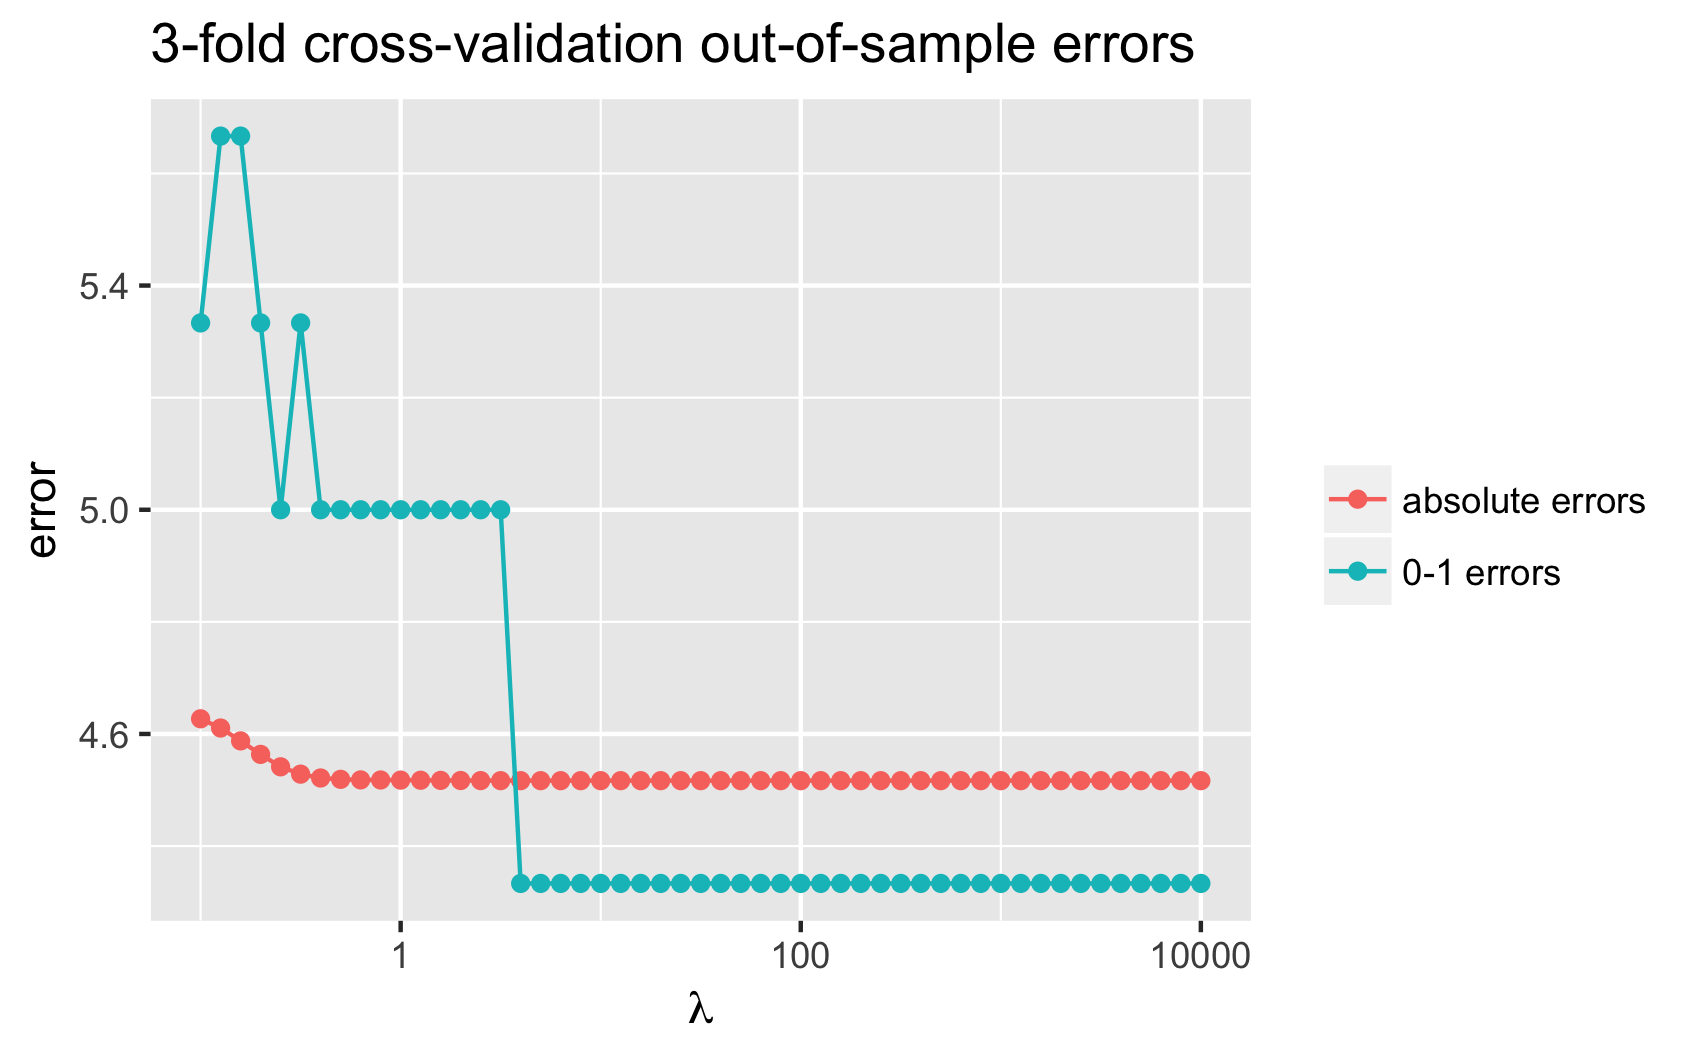
\includegraphics[scale=0.2]{3-fold-CV-kegg.png}
\caption{\label{fig:one}Error using the grouped data versus the LASSO penalty $\lambda$.
In blue, the mean 0-1 error on the held-out set. In red, the mean absolute error on the held-out set.}
\end{center}
\end{figure}

By the ``eye test'' -- we used only 3 folds, so it seems foolish to use the ``most parsimonious within one standard 
error'' trick simply by having a not-believable estimate of the standard error -- the absolute error seems to not 
improve for $\lambda > 10^{-0.4}$ while the 0-1 error does not improve for $\lambda > 10^{+0.6}$. Using the more
restrictive value $\lambda = 10^{+0.6}$, running on the entire grouped data set shows that the predicted values 
$\hat{y}$ are all below 0.5, indicating that the rounded predictions would all be zero! See Figure \ref{fig:two}

\begin{figure}[h]
\begin{center}
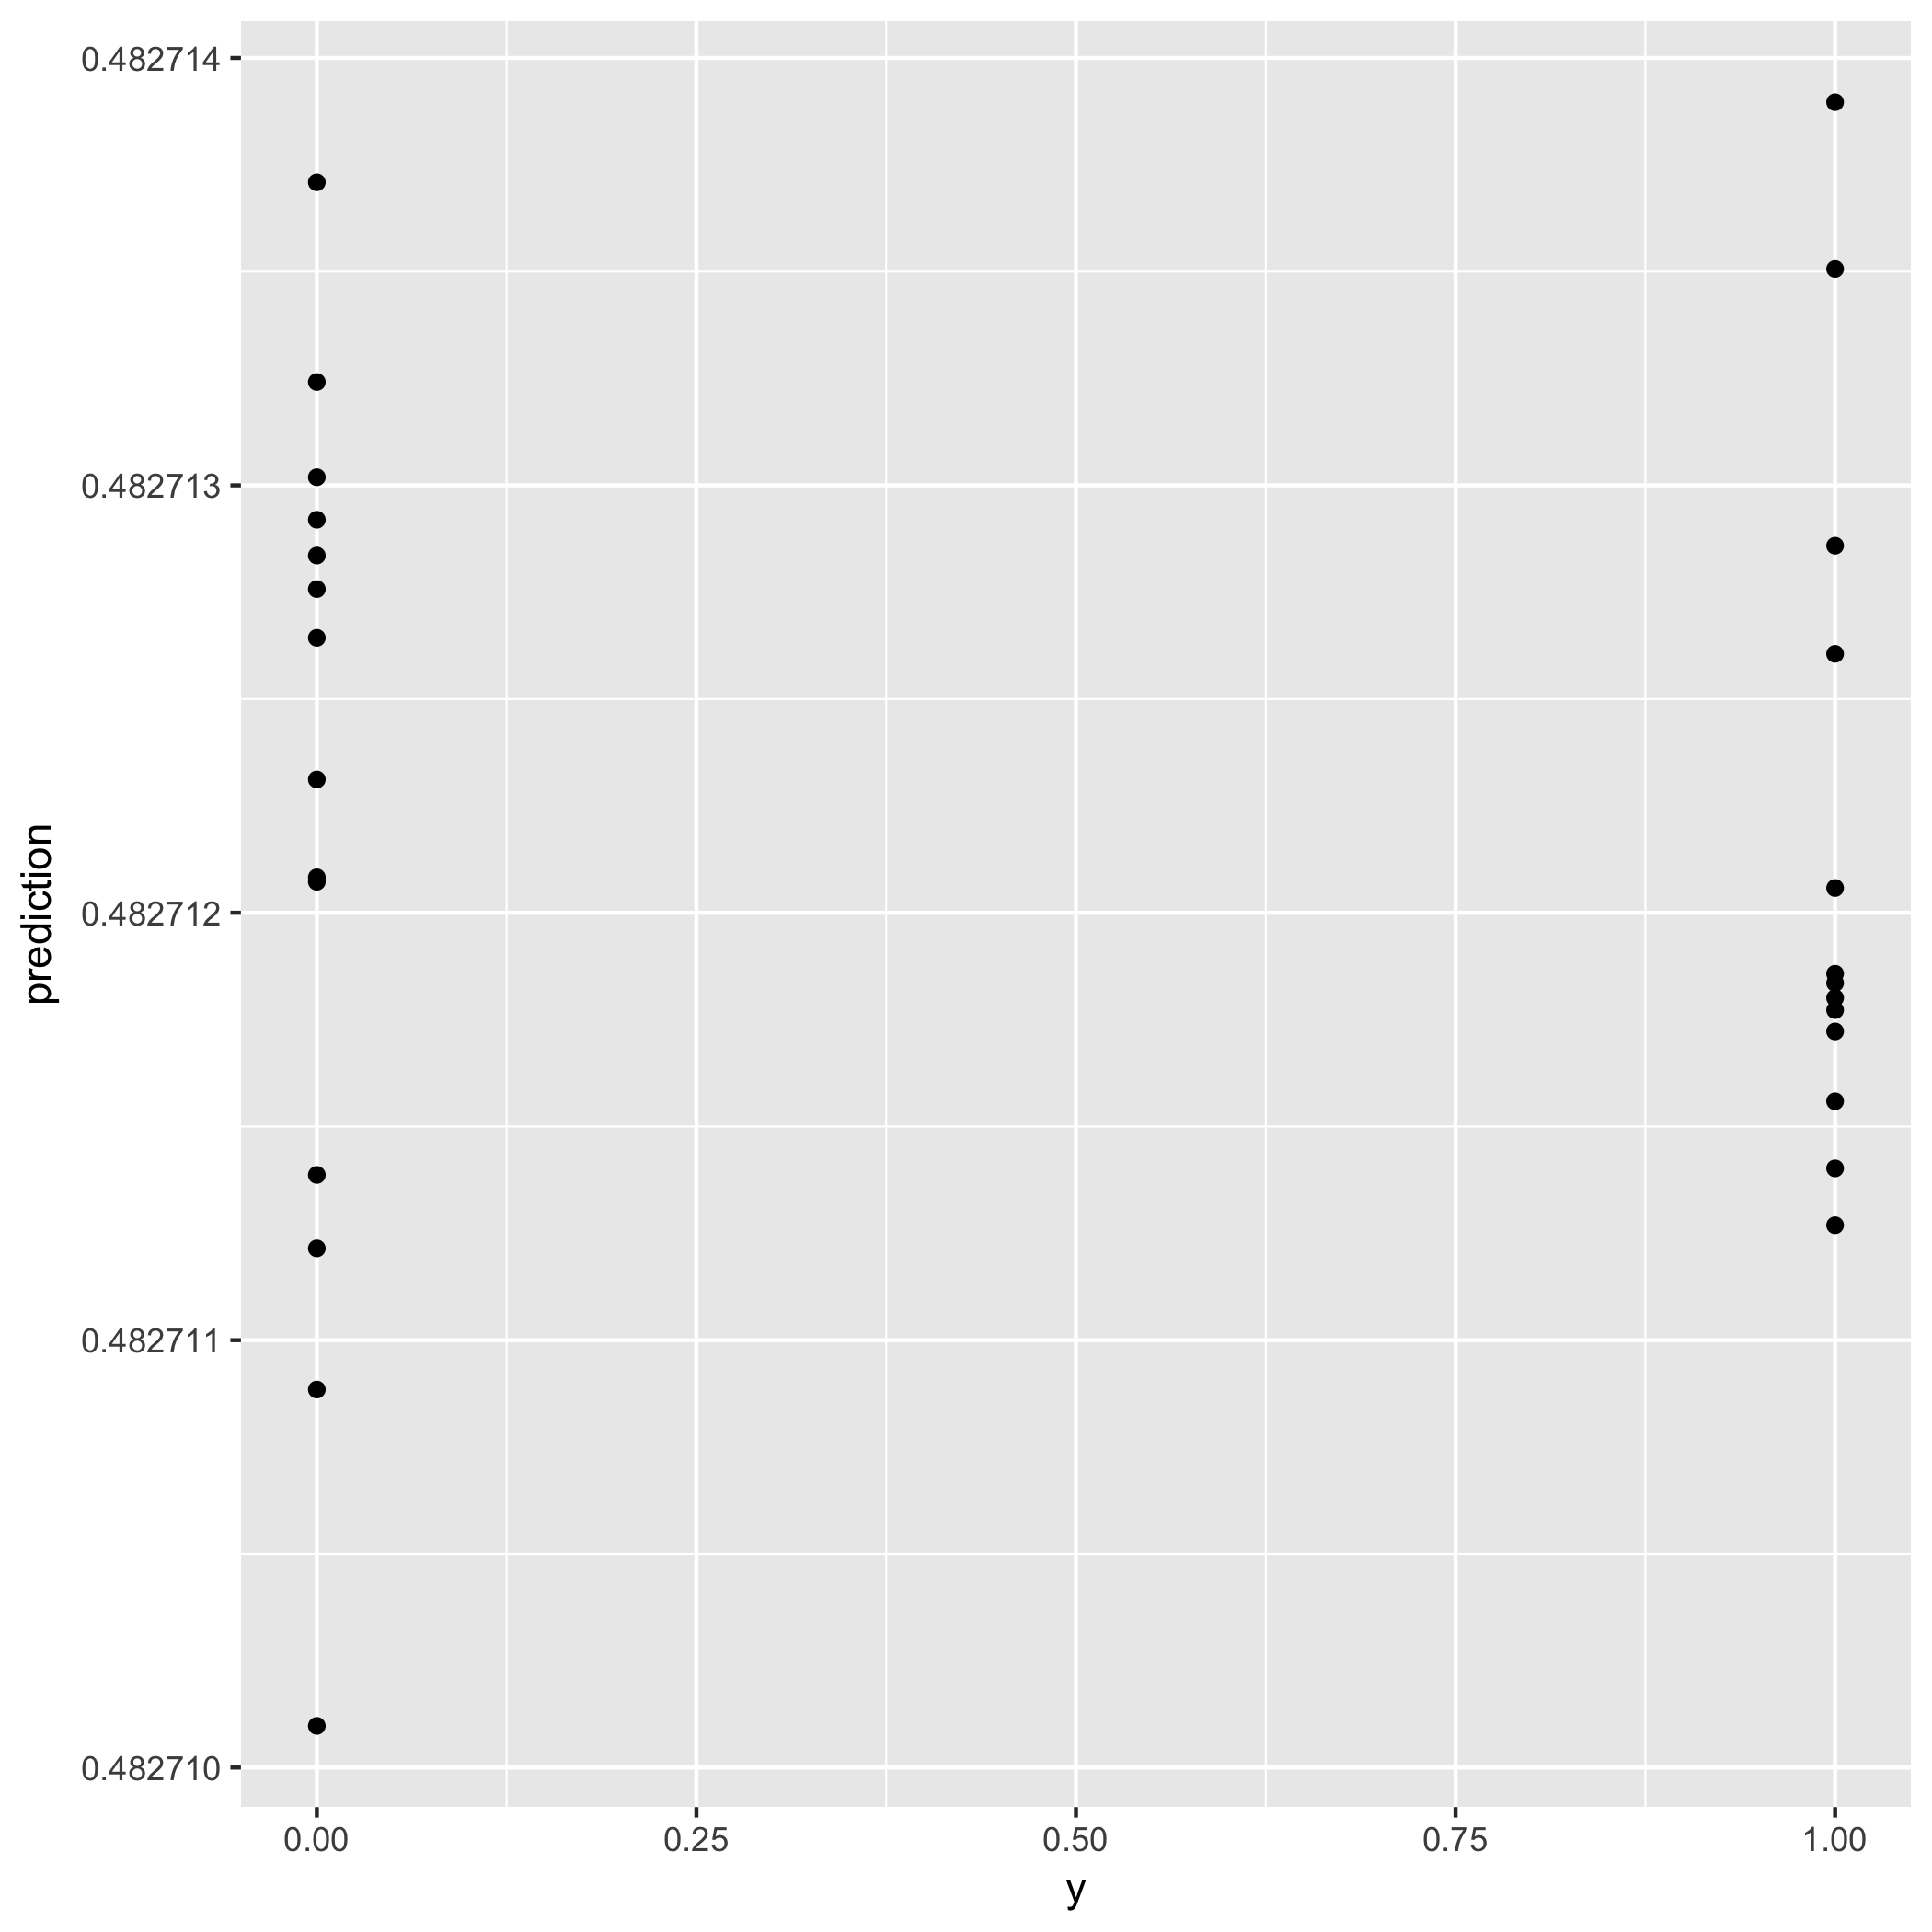
\includegraphics[scale=0.1]{kegg-cv-prediction.png}
\caption{\label{fig:two}Predictions for $\lambda=10^{+0.6}$ on the grouped data set versus actual value (0 for control, 1 for treatment).}
\end{center}
\end{figure}

Out of $\tilde{P}=2227$ possible gene groups, this process produced non-zero coefficients for only 4. For the $P=152448$ total genes, the same process (for $\lambda=10^{+0.5}$) produced 25 non-zero coefficients. The gene groups are included in Table \ref{tbl:groups}, but should not be viewed as particularly reliable, for the reasons outlined above.

On the grouped data, we also tried using the raw counts. The cross-validated error plot was certainly more 
interesting, but the results were similar, where the predictions using the entire grouped data set were abysmal.

\subsection{\texttt{DESeq2}}
The R package \texttt{DESeq2} is a standard for analyzing this kind of data. It uses the model below to identify
which genes are more indicative of a control or treatment sample:
\begin{align*}
X_{i,j}\sim& \textrm{Negative-Binomial}(\mu_{i,j}, \alpha_i)\\
\mu_{i,j}=&s_jq_{i,j}\\
\log_2(q_{i,j})=&u_{j,\cdot} \beta_i
\end{align*}
where $u_{j,\cdot}$ comes from the $N\times 3$ design matrix (first column all ones, second column as an indicator
for being in the control group, third column for being in the treatment group), and $\beta_i$ is the quantity of interest,
with $\gamma_i=\beta_{i, 3}-\beta_{i,2}$ being the ``log2 fold change.'' We won't discuss the other parameters
here as they are not of interest in this analysis. For more information, see \S4.1 of \citep{deseq2}.

It's a little unclear exactly how \texttt{DESeq2} handles multiple testing. It says that it uses the Benjamini-Hochberg
procedure to create adjusted $p$-values (such that checking $\textrm{padj}_i<\alpha$ is equivalent to the
Benjamini-Hochberg procedure with FDR controlled at $\alpha$) \citep{benjamini1995controlling}. 
Any gene (gene group) with such an adjusted $p$-value is included in Table \ref{tbl:genes} (Table \ref{tbl:groups}).
However, this 
adjusted $p$-value is not always available -- in cases where a gene/group is filtered by ``independent filtering'' (having a low
mean normalized count),
it is set to \texttt{NA}. See \S1.5.3 of \citep{deseq2} for details on this procedure.

So, we implemented our own, standard version of the Benjamini-Hochberg procedure
on the non-adjusted $p$-values (that are the result of a Wald test for the log2 fold change). While in principle,
the genes identified in this manner need not have been a subset of those identified in the default setting,
in practice they are. These are seen in the ``Our B-H'' column in the tables.

Finally, we also looked into the ``independent filtering'' which is described in \S3.8 and \S4.7 of \citep{deseq2}.
This essentially tries to determine a cutoff for the mean of the normalized counts where smaller values are
excluded from the analysis. Turning this off (in general) will likely yield fewer rejections once \texttt{DESeq2}'s 
internal Benjamini-Hochberg procedure is applied -- more ``noise'' data will enter in, padding the ``signal'' data,
making it more difficult for a particular signal to make it past the Benjamini-Hochberg procedure (if the significance
level is kept constant). However, if we are happy with fewer rejections (perhaps just a smaller set of genes
to consider during an initial investigation), this becomes useful. The results from turning off the filtering (but using
\texttt{DESeq2}'s specialized Benjamini-Hochberg procedure) are in the ``No Filtering'' column in the tables.




\section{Results}
\begin{table}[!h]
\begin{center}
\begin{tabular}{r|cccl}
Gene group & LR & \texttt{DESeq2} & Our B-H & No Filtering\\
\hline
1.1.1.36 & & - & & \\
1.14.-.-   & & - & &\\
1.14.14.- & & - & & \\
1.14.14.10& & - & -&- \\
1.2.1.39& & - & -& -\\
1.2.99.8& & - & -& -\\
1.3.99.5& & - & -& -\\
1.4.99.-  & Y \\
2.1.1.140& & - &- &- \\
2.7.7.73& & - & & \\
2.7.13.3 & Y \\
3.1.3.21& & - & -& -\\
3.4.11.-& & + & +& +\\
3.4.11.9 & Y \\
3.4.24.-  & Y\\
3.5.1.54& & - & -& -\\
3.6.3.9& & + &+& +\\
4.2.1.153& & - & & \\
5.1.1.7& & - & -& -\\
5.3.3.-& & - &- & -\\
5.4.99.26& & - & -& -\\
6.-.-.-& & - & & \\
6.3.3.3& & - &- &- \\
6.4.1.6& & - & &- \\
\end{tabular}
\caption{\label{tbl:groups}Gene groups identified using the various strategies outlined. A ``Y'' in the first column
indicates that the listed gene group had a non-zero coefficient in the logistic regression method -- this is primarily
recorded for posterity, not because the analysis is trusted. For the remaining columns, a ``-'' indicates that
a high count in that gene group is indicative of being a control sample. A ``+'' indicates that a high count is indicative
of being a treatment sample. A blank indicates that it is not present in that particular model.}
\end{center}
\end{table}

\begin{table}[!h]
\begin{center}
\begin{tabular}{r|ccc}
Gene &  \texttt{DESeq2} & B-H & No Filter\\
\hline
abau\_c\_1\_3356 & - &  &   \\
aisr\_c\_20\_1998 & -  &  &   \\
   amas2385\_c\_4\_872 & - &  &   \\
   aot170\_c\_17\_1854 & - &  &   \\
  aot171\_c\_140\_1750 & - &  &   \\
     aot171\_c\_3\_100 & - &  &   \\
   aot172\_c\_99\_1663 & - &  &   \\
   aot448\_c\_6\_964 & +  &  &   \\
  apre\_c\_1\_700 & - &  &   \\
 cdip\_c\_1\_1509 & - &  &   \\
chom\_c\_27\_1386 & - &  &   \\
chom\_c\_55\_2086 & - &  &   \\
  cper\_c\_2\_296   & +  &  &   \\
 cure\_c\_1\_1578 & - &  &   \\
    dpig\_c\_1\_8   & +  &  & +  \\
     efae1080\_c\_1\_913 & - &  &   \\
     esak\_c\_1\_3901 & - &  &   \\
    fnucp\_c\_3\_1442  & + &  &   \\
  fper2555\_c\_2\_652   & +  &  &   \\
   gmor\_c\_19\_1592 & - &  &   \\
 lcat\_c\_18\_1871 & - &  &   \\
    lgas\_c\_1\_25 & - &  &   \\
  lgoo\_c\_14\_911 & - &  &   \\
   lmon\_c\_1\_308 & - &  &   \\
lot107\_c\_9\_1346  &+ &  &   \\ 
  mlot\_c\_1\_5349 & - &  &   \\
  mneo\_c\_1\_1226 & - &  &   \\
  mneo\_c\_1\_1611 & - &  &   \\
  mot186\_c\_3\_1980 & - &  &   \\
      mtub\_c\_1\_788   &+ &  &   \\
      nbac\_c\_3\_267 & - &  &   \\
 NCBIABIX\_c\_1\_1199 & - &  &   \\
opro\_c\_21\_2166 & - &  &   \\
  pend\_c\_1\_176 & - &  &   \\
peno\_c\_75\_2748 & - &  &   \\
pmel\_c\_20\_1104 & - &  &   \\
 pmuls\_c\_6\_923 & - &  &   
     \end{tabular}
  \begin{tabular}{r|ccc}
Gene &  \texttt{DESeq2} &   B-H & No Filter\\
\hline
 pot786\_c\_28\_1621 & - &  &   \\
 pple\_c\_7\_1120 & - &  &   \\
 pstu\_c\_1\_2331 & - &  &   \\
pver\_c\_10\_1377 & - &  &   \\
  raer\_c\_1\_313 & - &  &   \\
raer\_c\_17\_1833 & - &  &   \\
  raer\_c\_2\_422 & - &  &   \\
 raer\_c\_5\_1016 & - &  &   \\
 raer\_c\_9\_1389 & - &  - & -  \\
  rden\_c\_1\_560 & - &  &   \\
    rden1994\_c\_1\_356 & - &  &   \\
    sked\_c\_1\_1556 & - &  &   \\
    sked\_c\_1\_1767 & -  &  &   \\
smal\_c\_1\_1545 & -  &  &   \\
smit\_c\_1\_1759 & -  &  &   \\
smut\_c\_1\_1468 & +  &  &   \\
smut\_c\_1\_1548 & +  &  &   \\
smut\_c\_1\_1794 & + &  &   \\
smut\_c\_1\_371 & +  &  &   \\
smut\_c\_1\_836 & +  &  &   \\
  sot138\_c\_21\_1472 & - &  &   \\
  sot149\_c\_17\_1639 & - &  &   \\
    ssal\_c\_18\_1887 & - &  &   \\
    tmed\_c\_12\_2247 & - &  &   \\
\end{tabular}
\caption{\label{tbl:genes}Genes identified using the various strategies outlined. The interpretation is identical
to that in Table \ref{tbl:groups}. The logistic regression data is not included here, because, like in the grouped data,
it is a) a completely different set of genes, and b) has seemingly no predictive power.}
\end{center}
\end{table}


Tables \ref{tbl:groups} and \ref{tbl:genes} represent the high-level results of this investigation. They indicate
genes/groups of genes identified by logistic regression (that should not be regarded highly for reasons outlined 
above) and by \texttt{DESeq2}. The variants applied to the latter indicate smaller subsets of genes/groups of genes
to consider when trying to investigate any biological basis for periodontal disease. In particular,
dpig\_c\_1\_8  and raer\_c\_9\_1389 seem indicative of positive and negative markers, respectively for disease based
on turning off \texttt{DESeq2}'s independent filtering (Table \ref{tbl:genes}). Information about the genes and groups
of genes discovered without using independent filtering can be found in Tables \ref{tbl:genes-info} and \ref{tbl:groups-info}.



\begin{table}[!h]
\begin{center}
\begin{tabular}{r|cccl}
Gene & Organism & Enrichment & Gene name & Gene function\\
\hline
dpig\_c\_1\_8 & D. pigrum & disease & pcrA & ATP-dependent DNA helicase\\
raer\_c\_9\_1389 & R. aeria & healthy & SAR0937 & Putative O-acetyltransferase
\end{tabular}
\caption{\label{tbl:genes-info}Information about genes identified without using independent filtering within \texttt{DESeq2}. This particular \emph{D. pigrum} gene appears to indicate disease while this \emph{R. aeria}
gene appears to indicate being healthy.}
\end{center}
\end{table}

\begin{table}[!h]
\begin{center}
\begin{tabular}{r|lll}
Gene group & Fold Change&Name & Class \\
\hline
1.14.14.10 & -2.0835574&nitrilotriacetate monoxygenase & oxidoreductase \\
1.2.1.39 & -1.7601778&phenylactaldehyde dehydrogenase & oxidoreductase \\
1.2.99.8 & -1.9174369&glyceraldehyde dehydrogenase & oxidoreductase \\
1.3.99.5 & -2.5358347&5alpha-reductase & oxidoreductase \\
2.1.1.140 & -2.4009629&(S)-coclaurine-N-methyltransferase & methyltransferase \\
3.1.3.21 &-2.6488779& glycerol 1 phosphatasae & hydrolase \\
3.4.11.- & 0.9773685&leukotriene-A4 hydrolase & hydrolase \\
3.5.1.54 & -2.0246868&allophanate hydrolase & hydrolase \\
3.6.3.9 &2.41233& Na/K ATPase & hydrolase \\
5.1.1.7 & -2.8294091&diaminopimelate epimerase & isomerase \\
5.3.3.- &-2.1665531& steroid isomerase & isomerase \\
5.4.99.26 & -1.648108&tRNA pseudouridine65 synthase & tRNA \\
6.3.3.3 & -2.5694759&dethiobiotin synthase & synthase 
\end{tabular}

\begin{tabular}{r|l}
Gene group & Function \\
\hline
1.14.14.10 &  synthesis of glyoxylate\\
1.2.1.39 &  synthesis of phenylacetate\\
1.2.99.8 &  synthesis of D-glycerate\\
1.3.99.5 &  steroid degradation\\
2.1.1.140 &  transfers methyl groups from coclaurine\\
3.1.3.21 & forms glycerol\\
3.4.11.- &  metalloprotease and aminopeptidase\\
3.5.1.54 &  catalyzes peptide bonds\\
3.6.3.9 & maintains membrane potential\\
5.1.1.7 &  lysine biosynthesis\\
5.3.3.- & 3-oxo-Delta4-steroid\\
5.4.99.26 &  modifies tRNA uridine65\\
6.3.3.3 &  synthesis of dethiobiotin
\end{tabular}
\caption{\label{tbl:groups-info}Information about gene groups identified without using independent filtering within \texttt{DESeq2}. The second column is the MAP estimate of the log2 fold change, which is positive when the group appears more indicative of treatment than control.}
\end{center}
\end{table}


\section{Discussion}
Of the 150,000+ observed genes in the analysis, only two showed to be statistically significant (see Table \ref{tbl:genes-info}). The pcrA gene, encoding the DNA helicase, was found to be upregulated in diseased samples. This protein is responsible for unwinding the tightly coiled DNA that occurs when a cell replicates. It is unclear what role this plays in disease progression, but the helicase may favor replication of diseased microbes and speed disease progression. The other gene, SAR0937, was found to be upregulated in healthy samples and encodes an acetyl-transferase. This protein is involved in amino acid synthesis, so diseased cells may alter available substrates to promote their growth.

In a similar analysis reducing genes to their KEGG pathways, enrichment was more common in healthy samples compared to diseased, showing that periodontitis, like many other diseases, has more than one path to a disease state. Despite the inherent complexity, the pathways that are enriched in the periodontal samples are particularly interesting. The most enriched gene, the Na/K ATPase (KEGG: 3.6.3.9), is responsible for maintaining the membrane potential inside the cell without which would cause a deleterious cellular environment and abnormal function. This balance is achieved by using energy from the hydrolysis of the molecule ATP to pump sodium and potassium against their concentration gradients into the cell. Upregulation of this gene could explain how microbes adapt in the low pH of the mouth and flourish in the diseased state. This ATPase comes at a fairly high energetic cost using about one-fifth of the cell's total energy, so it's striking that despite this energy cost, the microbes chose to upregulate, perhaps compensating for loss of energy elsewhere. The other enriched enzyme is a leukotriene hydrolase. Interestingly, this protein contains aminopeptidase activity indicating that it is involved in breaking proteins into smaller amino acid subunits. It has been reported previously that changes in microbiota in diseases alter their metabolism by scavenging amino acids for a different metabolic use. Evidence of this in our analysis gives credence to this finding.

The majority of gene products found in this analysis showed a downregulation in the diseased samples.  The two major protein classes involved in this downregulation are oxidoreductases and hydrolases. Oxidoreductases transfer electrons from one molecule to another, and in this instance, probably helps the microbiota to adapt to a diverse environment. Hydrolases in general cleave chemical bonds using water. Though it is difficult to tease apart each hydrolases role in promoting periodontitis, it is important to note that a shift in metabolism would require different molecular substrates, and thus changes in these molecules are observed.

Diseased phenotypes in microbiomes adapt by changing their metabolism and promoting a more favorable growth environment. Our findings give support to this idea as genetic shifts to better maintaining cellular membrane potential and modifying substrate amounts for various metabolic processes are observed. Further work in this analysis would involve integrating species level abundance to observe not only the genetic changes associated with periodontitis but how the microbial community as a whole is changed. Additionally, with more data, we could make a more meaningful attempt to elucidate the progression (rather than presence) of periodontis, also controlling better for within-subject variation (or lack thereof) in the analysis.



\bibliographystyle{plainnat}
\bibliography{/Users/Evan/GitProjects/tex-docs/references}

% If using biblatex
% \printbibliography

\end{document}